
\chapter{Introduction}

While major parts of the functionality of {Subset 026} are developed in 
higher-level languages, there is also a substantial part of \emph{supporting} software
that is developed in the programming language~C.

In this document we report about \emph{preliminary} results on the verification
of C-code developed in the OpenETCS project.
In particular, we report on the use of static analysis methods (including formal methods)
on C code that has been developed by the project partner Siemens (Germany).
Figure~\ref{fig:Bitwalker-Overview} gives an overview on the software that
is in the focus of this report.

\begin{figure}[hbt]
\begin{center}
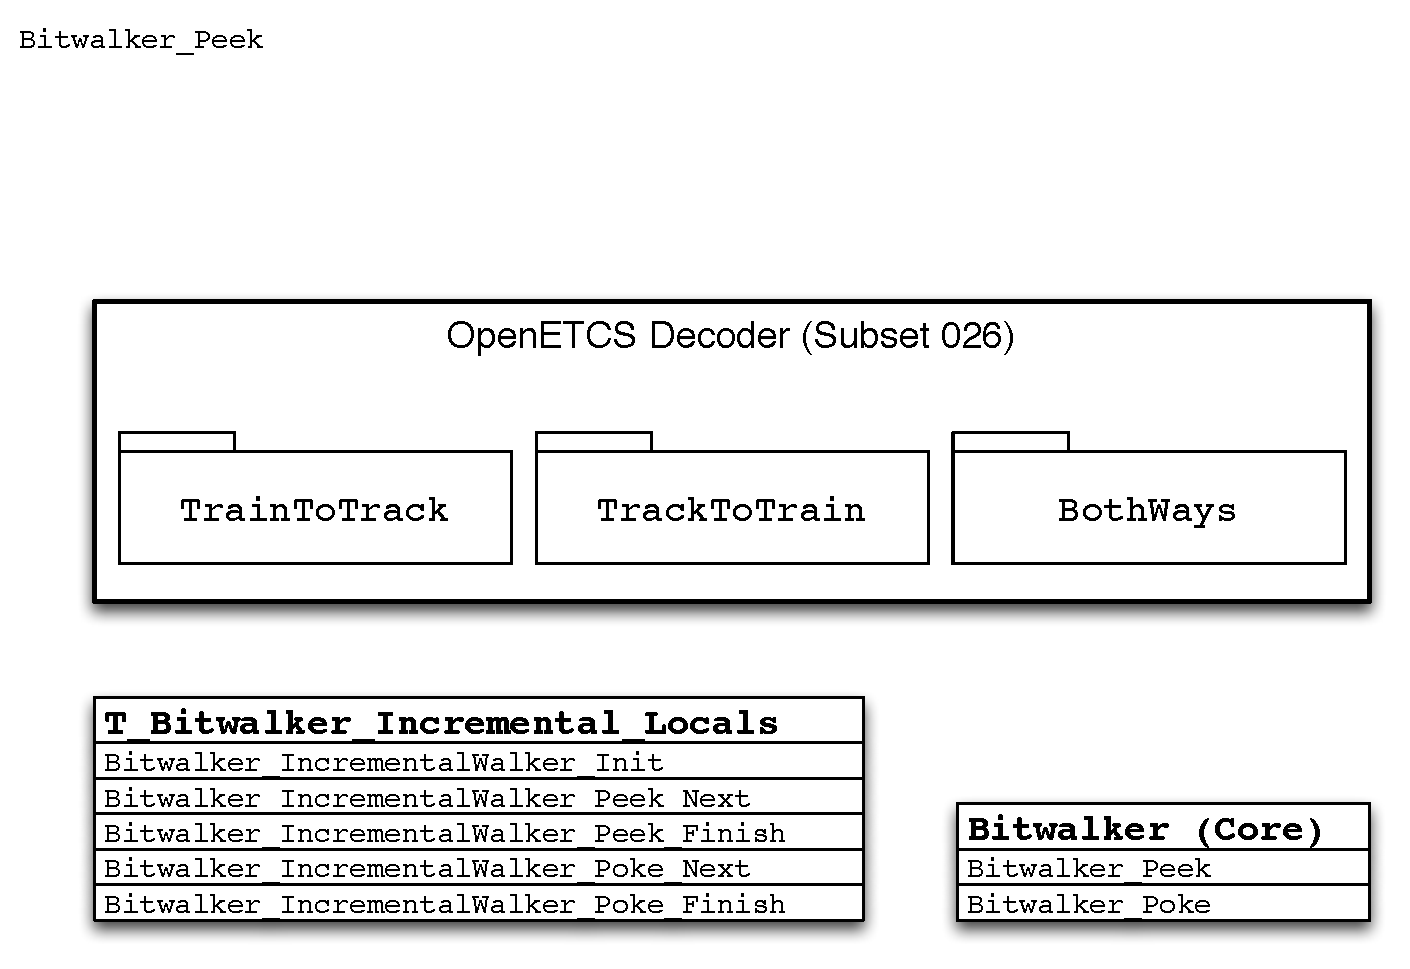
\includegraphics[width=0.8\textwidth]{figures/Bitwalker-Overview.pdf}
\caption{\label{fig:Bitwalker-Overview} The place of \texttt{Bitwalker} with the OpenETCS software}
\end{center}
\end{figure}

The OpenETCS decoder is a large collection of functions dedicated to
the reading of of ETCS messages.
In order to fulfill their task these function rely on the relatively
small software package \inl{Bitwalker}.
The \inl{Bitwalker} software, as seen by the OpenETCS decoder,
is best understood as a ``class'' with a handful of methods.
Note that this class is implemented in~C as a \inl{struct} where
the methods are implemented as functions.
The core functionality  of this class, which consists in converting bit sequences to integers
and the other way round, depends on two more basic function, namely~\peek and~\poke.

This software has been analyzed by the OpenETCS project partners SQS (Spain)
and Fraunhofer FOKUS (Germany).
The Frama-C tool, which is developed by the French project partner {CEA LIST},
has been used for some of the analyses.

\clearpage

The ultimate verification goals are the following

\begin{enumerate}
\item provide evidence that the Bitwalker software satisfies 
      accepted quality standards
\item develop a formal specification for the Bitwalker software
\item verify that the Bitwalker software satisfies its formal specification
\item show that the Bitwalker software does not raise runtime errors
\item verify that OpenETCS decoder calls the Bitwalker software only
      according to its specification
\end{enumerate}

We are confident that all these verification goals can be reached.
For this preliminary verification report, report,
we only provide partial answers to the first four topics.
In order to achieve the last goal more development and verification
work is currently conducted by Fraunhofer ESK and Fraunhofer FOKUS. 

\section*{Structure of this Document}

Section~\ref{sec:frama-c} gives a short overview on the \framacwp tool
that plays a central role in the verification of the Bitwalker functions.
Here we also try to rectify some misunderstandings about formal verification
that we have encountered in our work.

In Section~\ref{sec:formal-verification} we analyze
the functions \peek and \poke from the Bitwalker core and
\begin{enumerate}
\item formally specify the
      expected functional behavior in the \acsl specification language of {Frama-C}
      and
\item using the {Frama-C} verification platform to establish a formal proof that these
      C~functions do not raise runtime errors when called according to their
      formal specification.
\end{enumerate}

In Section~\ref{sec:static-analysis} we report about the results of a broad range
of static analyses. 
These methods are aimed at finding well-known quality deficiencies that
might occur in C or \CC\ software.

Thus, so far only a part of Siemens' \emph{BitWalker} has been formalized and verified.
In the process of this work several enhancements for the \framac verification platform
have been identified and reported to the developers at {CEA LIST}.

In Section~\ref{sec:conclusions} we draw preliminary conclusions
and outline the next steps in our verification efforts.

